%!TEX root = main.tex

\chapter{Problema de $t$-spanner de peso mínimo}
\label{cap:mwsp}

Neste capítulo apresentamos uma formulação linear inteira que
propusemos para o problema de $t$-spanner de peso mínimo (MWSP).


\section{Poliedro dos $t$-spanners de um grafo}

No problema do $t$-spanner de peso mínimo (MWSP), dado um grafo
$G=(V,E)$ com peso \hbox{$w: E \to \espacoRpos$,} e um número real
$t \ge 1$, queremos encontrar um conjunto $F \subseteq E$ de peso
mínimo tal que $G[F]$ é um $t$-spanner de $G$.  Para isso, definimos o
poliedro dos $t$-spanners de $G$, objetivando usar técnicas de
programação linear para encontrar uma solução ótima. Esse poliedro é
assim definido.
%
\begin{equation*}
\begin{split}
P_{span}(G,t) := \text{conv}\{\incid^{F} \in \espacoE, F \subseteq E\; |\; \text{$G[F]$ é um $t$-spanner de $G$\}}. 
\end{split}
\end{equation*}

Observe que se $t'' \ge t' \ge 1$, então $P_{span}(G,t') \subseteq P_{span}(G,t'')$.


\smallskip

\subsection{Dimensão do poliedro}
\label{sec:dim_poliedro}

%% No que segue, referimo-nos a um grafo $G=(V,E)$ e a um real fixo $t \ge 1$.
%% Para $u,v \in V$, denotamos por $\PathuvG$ a coleção de caminhos
%% $t$-spanner em $G$  que vai de $u$ a $v$.
%% Dizemos que uma aresta $f \in E$ é uma 
%% \emph{aresta $t$-essencial} 
%% %\emph{ponte $t$-spanner} 
%% de $G$ se $G-f$ não é $t$-spanner de $G$. 
%% Seja \\
%% \centerline{$\BridgeG = \{e \in E\; |\; e$ é uma aresta $t$-essencial de $G\}$.}
Seja $\BridgeG = \{e \in E\; |\; e$ é uma aresta $t$-essencial de $G\}$. Lembramos que uma aresta $e$ de $G$ 
é $t$-essencial se $G-e$ não é um $t$-spanner de $G$. 

No que segue, supomos que $|E|=m$, $E=\{e_1, \ldots, e_m\}$ e que os
vetores $x\in \espacoE$ estão indexados por $E$, ou seja,
%% $x=(x_{e_1}, \ldots, x_{e_m})$. Também escrevemos $x(e)$ em vez de $x_e$.
$x=(x_{e_1}, \ldots, x_{e_m})$.
%% Para $F\subseteq E$, denotamos por $\incid^{F}$ o vetor de incidência de~$F$.


\begin{lema}
$dim(P_{span}(G,t)) = |E| - |\BridgeG|$.
\begin{proof}
Seja $f \in \BridgeG$. Então, para cada $\incid^{F} \in P_{span}(G,t)$, segue que 
$f \in F$. Sendo assim, $P_{span}(G,t) \subseteq \{x \in \espacoE | \, x_f = 1\}$. Logo, 
$dim(P_{span}(G,t)) \le |E| - |\BridgeG|$.

Como $G$ é $t$-spanner, $\incid^{E} \in P_{span}(G,t)$ e 
$\incid^{E-f} \in P_{span}(G,t), \forall f \in E \setminus
\Bridge$. Claramente tais vetores são afim-independentes, e portanto, 
$dim(P_{span}(G,t)) \ge |E| - |\BridgeG|$. 
\end{proof}
\end{lema}

\section{Outro poliedro associado ao poliedro dos 
  \hbox{$t$-spanners}}
\label{sec:formulacao}

 Para $G' = (V, E') \subseteq G = (V,E)$, denotamos por
 $\PathuvGprime$ a coleção de caminhos
 $t$-spanner entre $u$ e $v$ que estão contidos em $G'$.
% %%
%Seja $\spanPath = \bigcup_{uv \in E} \PathuvG$ a coleção de caminhos
%$t$-spanner entre todos os pares de vértices que definem aresta em $G$.

Para obter uma descrição do poliedro $P_{span}(G,t)$ definido na seção anterior,
introduziremos um outro poliedro, e mostraremos como esses dois poliedros esstão relacionados. 

Para definir esse novo poliedro, faremos uso de dois tipos de
variáveis de decisão $0/1$: (a)~variável $x \in \espacoE$ com o
seguinte significado: para cada $e \in E$, $x_e = 1$ se e só se $e$
faz parte da solução $F$; (b) variável $Y \in \espacoY$, para impor a
condição de existência de caminhos $t$-spanner para cada aresta $e=uv$
de $G$. Para conseguir isso, impomos a existência de um caminho
$P \in \PathuvF$, onde $F \subseteq E$ é o conjunto das arestas
selecionadas.


As três primeiras restrições do sistema abaixo, juntamente com a
restrição de que $x$ e $Y$ são variáveis 0/1, capturam exatamente isso
que desejamos.  (Para cada aresta $e=uv$ em $G$, garantimos a
existência de um caminho $P$ em $\PathuvF$ que é $t$-spanner, e para o
qual temos que $Y_{e,f} = 1$ para toda aresta $f \in E(P)$.)  Nessa
descrição, para $W \subset V$, denotamos por $\delta(W)$ o conjunto
das arestas de $G$ que têm uma extremidade em $W$ e outra em
$\overline W$ (ou seja, $\delta(W)$ define um corte em $G$).  Além
disso, para $F \subseteq E$, $Y_{e,F}$ denota a soma
$\sum_{f \in F}Y_{e,f}$.

\smallskip


Considere o seguinte sistema linear, no qual está  relaxada a condição de integralidade
das variáveis. 

%% \newpage

\begin{lpformulation}[\PGtrestricoes]
\lpeq[res_mmst:path]{Y_{e,\delta(W)} \ge 1}{e \in E,\, \forall \,W \subset
  V \,\hbox{com}\, e\in \delta(W)}
\lpeq[res_mmst:relate_vars]{Y_{e,f} \le x_f}{e,f \in E}
\lpeq[res_mmst:spanner]{\sum_{f \in E}Y_{e,f} w_f \le  t \cdot w_e}{e \in E}
\lpeq[res_mmst:int_x]{0 \le x_e \le 1}{e \in E}
\lpeq[res_mmst:int_Y]{0 \le Y_{e,f} \le 1}{e,f \in E}
\end{lpformulation}



$$P(G,t)= \{(x, Y)\; |\; x \in \espacoE, Y \in \espacoY \text{ e } (x,Y) \text{ satisfaz } \PGtrestricoes\}.$$

% Ao longo desta seção, iremos provar que o fecho inteiro da projeção de 
% $P(G,t)$ em no espaço das variáveis $x$ é igual ao poliedro $P_{span}(G,t)$.

\medskip

Seja $(P(G,t))_{I}$ o fecho inteiro do poliedro $P(G,t)$. Veremos a seguir 
como $P_{span}(G,t)$ e  $(P(G,t))_{I}$ estão relacionados.
%

% Vamos primeiramente provar que a cada vértice em $P_{span}(G,t)$ 
% corresponde um vértice na projeção de $(P(G,t))_{I}$
% no espaço das variáveis $x$ (veja o Fato
% \ref{afirm:sol_viavel_lp}). Depois, iremos provar a recíproca: a  cada
% vértice da projeção de $(P(G,t))_{I}$ no espaço das variáveis $x$,
% corresponde  um vértice $\incid^{F} \in P_{span}(G,t)$ (veja os 
% Fatos~\ref{afirm:sol_viavel_Pspan} e \ref{corol:Y_suporte_minimo}),
% garantindo assim que esses poliedros são iguais (veja a 
% Proposição~\ref{prop:equivalencia_poliedros}). 

%%%%%%%%%%%%%%%%%%%%%%%% 


Note que no programa linear $\PGtrestricoes$ não há variáveis diretamente associadas
aos caminhos que respeitam a restrição de $t$-spanner, como é comum
ocorrer nas modelagens tradicionais~\cite{SigurdZ2004,DinitzK2011}. 
No lugar de variáveis associadas a caminhos, usamos a variável~$Y$
(indexada por pares de arestas). 

Seja $(x,Y)$ um ponto inteiro de $P(G,t)$ e $H$ a solução associada a
$(x,Y)$, definida como $H= G[F]$, onde $x=\incid^{F}$. 
A restrição (\ref{res_mmst:relate_vars}) 
diz que para $f \in E$, se $Y_{e,f} = 1$ para algum $e \in E$, então $f$ 
deve fazer parte da solução $H$. Além disso, se $f \in E$ 
não faz parte da solução $H$, então não existe $e \in E$ tal que $Y_{e,f} = 1$. 
%Em outras palavras, $E(G') \subseteq E(H)$. 

Pelo Lema~\ref{lem:definicoes} é suficiente garantirmos que 
a condição de caminho $t$-spanner está satisfeita pelos pares de vértices 
$u,v \in V$ tais que $uv \in E$. Por essa razão, apenas para cada aresta definimos 
variáveis da forma $Y_{e,f}$, para cada $e,f \in E$. 

Note que, nesta formulação, a menos das
restrições~(\ref{res_mmst:path}), há apenas um número polinomial de restrições no tamanho de $E$.
Veremos mais adiante que as restrições~(\ref{res_mmst:path}) podem ser
separadas em tempo polinomial (no tamanho de $V$).

A proposição a seguir mostra que a todo vértice de $P_{span}(G,t)$
corresponde um vértice de  $(P(G,t))_{I}$. 


\begin{proposicao}  %%%% new  -- era fato %%%%%%%%%%%%%%%%%%%%%
\label{afirm:sol_viavel_lp} 
Seja  $x'$ um vértice de $P_{span}(G,t)$. Então existe $Y'$
tal que $(x', Y')$ é um vértice de $(P(G,t))_{I}$. 
\begin{proof}

  Seja $x' = \incid^{F}$ um vértice de $P_{span}(G,t)$ associado ao $t$-spanner $G[F]$. 
Para cada $e=uv \in E$, considere um caminho $P_{u,v} \in \PathuvF$. 
%o caminho mínimo numerado entre $u$ e $v$ em $G[S]$.
%Para cada $e = uv, f \in E$, 
Defina $Y'\in \espacoY$ da seguinte forma: 
 \begin{align*}
% \forall e \in E,\; x'_e &= \incid^{F}_{e} \\
 \forall e=uv \in E, f \in E,\;\; Y'_{e,f}  &=
\begin{cases}
    1& \text{se $f \in E(P_{u,v}),$} \\
    0& \text{caso contrário.}
    %0& \text{se $f \in E \setminus E(P_{u,v}).$}
\end{cases}
\end{align*}

Claramente, $(x, Y')$ satisfaz todas as restrições do sistema
\PGtrestricoes, e como este é um vetor $0/1$, segue que é um vértice de
$(P(G,t))_{I}$. 

Note que, pode haver  vetores $Y''$ distintos de $Y'$ para os quais
$(x', Y'')$ são vértices de $(P(G,t))_{I}$. 

\end{proof}
\end{proposicao}  %%%%%%%%%%%%%%%%%%%%%%%%%%%%%%%%%%%%%%

A proposição a seguir mostra que a todo vértice de $(P(G,t))_{I}$ 
corresponde um vértice de $P_{span}(G,t)$. 

\begin{proposicao}  %%%%%%%%%%%%%%%%%%%%%%%%%%%%%%%%%  
\label{prop:correct_form}
Seja %$Sol = 
$(x',Y')$ um vértice de $(P(G,t))_{I}$.  %uma solução ótima de \ref{lp:primal_mwsp} 
Para $e \in E$, seja $F(e) = \{f \in E\; |\; Y'_{e,f} = 1\}$. 
Seja $E_{x'} = \{e \in E\; |\; x'_e = 1\}$ e $H = G[E_{x'}]$. 
Então

\begin{itemize} %[label=(\alph*)]
\item[{\rm (a)}] %\label{prop:Yuv_caminho}
Para cada aresta $e = uv \in E$, existe um caminho $P$  entre $u$ e $v$ em 
$G[F(e)]$ para o qual $Y'(e,f) = 1$ para todo $f\in E(P)$. 

 % Além disso, $G[F(e)]$ é um caminho entre $u$ e $v$.

\item[{\rm (b)}]%\label{prop:gerador_conexo_G}
  O subgrafo $G' = G[\bigcup_{e \in E}F(e)]$ é gerador e conexo.


\item[{\rm (c)}] % \label{corol:standard_spanner}
%\label{prop:x_spanner}
$H$ é um $t$-spanner de $G$, e portanto $x'$ é um vértice de $P_{span}(G,t)$.
\end{itemize}

\begin{proof}

  Prova do item (a).
  % 
  Seja $e = uv \in E$. Suponha,  por absurdo, que não exista um 
  caminho entre $u$ e $v$ em $G[F(e)]$. Então $u$ e $v$ estão 
  em componentes distintas em $G[F(e)]$. Seja $G_u$ o grafo induzido pelos 
  vértices da componente de $G[F(e)]$ que contém $u$. Seja $W = V(G_u)$. Mas 
  então a restrição~(\ref{res_mmst:path}) é violada pelo par $e$, $W$, 
  contradizendo a hipótese de que $(x',Y') \in P(G,t)$. Concluímos
  então que deve existir um caminho $P$ entre $u$ e $v$ em $G[F(e)]$
  para o qual  $Y'(e,f) = 1$ para todo $f\in E(P)$. 

\medskip

\noindent Prova do item (b).
%
Sejam $u,v \in V$. Como $G$ é conexo, existe um caminho $P$ entre $u$ e
$v$ em $G$, digamos 
\mbox{$P = (u = u_0, u_1,\ldots, u_{l-1}, u_l = v)$}. 
Pelo item~(a)  e sabendo que $G[F(e)] \subseteq G'$, 
para cada $e=u_{i-i}u_{i} \in E(P)$, existe um caminho entre $u_{i-1}$ e 
$u_{i}$ em $G[F(e)]$, e portanto em $G'$. 
Sendo assim, $u$ e $v$ estão conectados em $G'$, donde segue que $G'$ é um 
subgrafo gerador conexo de $G$.

\medskip

\noindent Prova do item (c).
Seja $e=uv \in E$.
Pelo item (a), temos que 
\mbox{$\dist_{G[F(e)]}(u,v) \leq  \sum_{f \in E}Y'_{e,f}\;w_f$}. 
Como valem os itens (a) e (b) e 
$G[F(e)] \subseteq G'$, temos que 
%é uma árvore (proposição \ref{prop:GY_arvore}), então 
\mbox{$\dist_{G'}(u,v) \le \dist_{G[F(e)]}(u,v)$}. 
Pela restrição~(\ref{res_mmst:relate_vars}) temos que $G' \subseteq H$; logo $H$ é subgrafo conexo e gerador de $G$.
Como  $(x',Y')$ respeita a restrição~(\ref{res_mmst:spanner}), segue que 
\begin{equation*}
\begin{split}
\dist_{H}(u,v) \le \dist_{G'}(u,v) \le \dist_{G[F(e)]}(u,v) \leq \sum_{f \in E} Y'_{e,f} \; w_f \le 
t \cdot w_e.
\end{split}
\end{equation*} 
A conclusão de que $H$ é um $t$-spanner de $G$ segue do
Lema~\ref{lem:definicoes}. Como $x'$ é o vetor de incidência de
$E(H)$, segue que  $x'$ é um vértice de $P_{span}(G,t)$.
\end{proof}

%\end{enumerate}
\end{proposicao}

% \begin{fato}
% \label{afirm:sol_viavel_Pspan}
% Um vértice $(x',Y') \in (P(G,t))_{I}$ tal que $Y'$ tem suporte minimal, corresponde a 
% um vértice $\incid^{F}$ de $P_{span}(G,t)$.
% %ótima de \ref{lp:primal_mwsp} corresponde a um vetor de $P_{span}(G)$.
% \begin{proof}
% Segue da proposição anterior. % \ref{corol:standard_spanner}.
% \end{proof}
% \end{fato}

% \begin{fato}
% \label{corol:Y_suporte_minimo}
% Para cada vértice $(x,Y) \in (P(G,t))_{I}$, existe um vértice  $(x,Y') \in (P(G,t))_{I}$ tal que $Y'$ tem suporte 
% minimal.
% % \begin{proof}
% % Podemos construir $(x,Y')$ utilizando construção semelhante à apresentada na prova 
% % da afirmação \ref{afirm:sol_viavel_lp}.
% % \end{proof}
% \end{fato}

Juntamos a seguir  os resultados das duas proposições anteriores.

\begin{proposicao}
   \label{prop:equivalencia_poliedros}
   As seguintes afirmações resumem como  $P_{span}(G,t)$ e $((P(G,t))_I$ estão relacionados:
   \begin{itemize}
     \item[{\rm (a)}] Se $x'$ é um vértice de $P_{span}(G,t)$, então existe $Y'$ (inteiro) tal que $(x',Y')$ é um vértice de $((P(G,t))_I$.
  \item[{\rm (b)}] Se $(x',Y')$ é um ponto inteiro que pertence a $P(G,t)$, então $x'$ é um vértice de $P_{span}(G,t)$.\\
    \end{itemize}
  \end{proposicao}  


 % \subsection{Uma formulação linear inteira para o  MWSP}
 
  Em vista do que foi provado anteriormente, o seguinte programa
  linear inteiro encontra uma solução ótima para o MWSP, com entrada $(G,w,t)$.

% Como abordado na seção \ref{sec:poliedro_sol_mmst}, para encontrar uma solução do MMST, 
% queremos descobrir o menor poliedro $P_x(G,t)$, para $t \ge 1$, o qual possui como 
% solução uma árvore. Encontrar uma árvore em $P_x(G,t)$ pode ser modelado através do 
% seguinte programa linear:

\begin{lpformulation}[(P)]
\lpobj*{min}{\sum_{e\in E} w_ex_e}
\lpeq*{(x,Y) \in P(G,t)}{}
\lpeq*{x\in\{0,1\}^{|E|}}{}
\lpeq*{Y \in\{0,1\}^{|E| \times |E|}}{}
%% \lplabel{lp:primal_mwsp} %tenho que comentar que está tendo conflito com hyperref
\end{lpformulation}
% Observe que uma solução ótima inteira de \ref{lp:primal_mwsp} com $|V| - 1$ arestas 
% é uma solução viável de MMST.

\begin{figure}[t] 
\centering
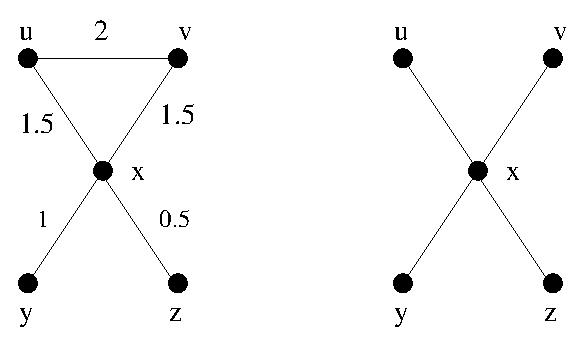
\includegraphics[scale=0.45]{figuras/exemplo_Y_minimal}
\caption{Um grafo com seu respectivo 2-spanner de peso mínimo}
\label{fig:exemplo_Y_minimal}
\end{figure}


% Na Proposição~\ref{prop:correct_form}~(a), %\ref{prop:Yuv_caminho}, 
% para $e = uv \in E$, 
% para mostrar que $G[F(e)]$ 
% é um caminho entre $u$ e $v$, nós assumimos como hipótese que $Y'$ possui 
% suporte minimal. Esta hipótese não é condição necessária para que uma solução 
% de (P) %\ref{lp:primal_mwsp}
% seja ótima.



% Considere a Figura \ref{fig:exemplo_Y_minimal}. Seja $G$ o grafo do lado 
% esquerdo da figura. Para $t = 2$, observe que a solução ótima de (P)
% \sisetup{round-mode=places,round-precision=1}
% corresponde à árvore no lado direito (para $t = \num{1,5}$, a solução também é
% \sisetup{round-mode=places,round-precision=2}
% $t$-spanner). 
% %, cujo fator de dilatação $t^*$ é $1.5$. 
% Seja $H$ esta solução. Para $u,v \in V$, seja $H_{u,v}$ o caminho entre
% $u$ e $v$ em $H$. 
% Vamos 
% construir uma solução viável $(x^*,Y^*)$ para (P) %\ref{lp:primal_mwsp}
% diferente de 
% $H$. Para cada $e=pq,f \in E$, defina $x^*$ e $Y^*$ da seguinte forma: 




% \begin{align*}
% x^*_e &= \incid^{H}_{e},\\
% Y^*_{e,f} &= 
% \begin{cases}
%     1& \text{se $f \in E(H_{p,q}),$}\\
%     1& \text{se $e = xy, f = xz,$}\\
%     0& \text{caso contrário.}
%     %% 0& \text{se $f \in E \setminus E(H_{p,q}).$}
% \end{cases}
% \end{align*}
% É fácil verificar que $(x^*,Y^*)$ é uma solução viável (ótima) de (P) %\ref{lp:primal_mwsp} 
% tal que $Y^*$ não tem suporte minimal.

% %% \subsection{Problema da separação}

\subsection{Separação das inequações de corte}
\label{sec:separacao}

Na formulação \PGtrestricoes, %\ref{lp:primal_mwsp},
o número de inequações correspondentes à 
restrição (\ref{res_mmst:path}) --- conhecidas como 
\emph{inequações de corte} ---  é exponencial no tamanho de $V$. 
%
%% No problema da separação, dado um conjunto de inequações e uma 
%% (possível) solução, nós queremos saber se existe uma inequação violada pela 
%% solução. 
%% Em outras palavras, desejamos saber se a solução é viável ou obter um 
%% certificado que corresponda a uma inequação violada. 
%mostra que a solução é viável ou exiba uma restrição violada.

A separação das inequações de corte %\ref{lp:primal_mwsp}
pode ser feita em tempo polinomial no tamanho de $V$. 
Dado um ponto  $(x^*, Y^*)$,   %\ref{lp:primal_mwsp}.
%Podemos interpretar a restrição \ref{res_mmst:path} da seguinte forma: 
para cada $e=uv \in E$, seja $G_{e} = (V, E')$, onde $E' = E$ e
$w_f:= Y^*_{e,f}, \forall f \in E(G_{e})$. A capacidade de um
$(u,v)$-corte mínimo em $G_{e}$ deve ser maior ou igual a $1$. Caso
exista um $e=uv \in E$ tal que um $(u,v)$-corte mínimo $\delta(W)$ em
$G_{e}$ tenha capacidade menor do que $1$, então o par $(e,W)$ é um
certificado de que a restrição~(\ref{res_mmst:path}) é violada. Como o
problema de encontrar um $(u,v)$-corte mínimo pode ser resolvido em
tempo polinomial (no tamanho do grafo), a 
separação para as inequações de corte pode ser feita em tempo polinomial
(veja \cite{KorteV2012}).
